\documentclass{book}

\usepackage{amsmath}
\usepackage{imakeidx}


\makeindex

\begin{document}

%%% frontmatter %%%
\frontmatter

\title{Angewandte Kryptographie}
\author{FH Campus Wien}
\date{SoSe 2025}

\maketitle
\tableofcontents

%%% mainmatter %%%
\mainmatter

\chapter{Effiziente Implementierungen}

%%% section %%%
\section{Langzahlen}

In (asymmetrischer) Kryptographie benötigen wir ülicherweise Werte, die weit größer sind, als die native Wortlänge der zugrundeliegenden Hardware.
Die meisten Register haben eine Wortlänge von 64 bit. Typische Schlüssellängen, beispielsweise für RSA Verschlüsselung, sind heutzutage 1024 bis 4096 bits.

\paragraph{Wie können solche Zahlen dargestellt werden?}

Eine Auswahl an Möglichkeiten ist:

\begin{enumerate}
    \item Residuen-Repräsentation \index{Residuen-Repräsentation}
    \item Verwendung von Arrays in nativer Wortgröße \index{Arrays mit nativer Wortgröße}
    \item Verwendung von Arrays kleiner als die native Wortgröße \index{Arrays kleiner als die native Wortgröße}
\end{enumerate}

\paragraph{Wie kann eine effiziente Modulo Reduktion implementiert werden?}

Die Division großer Zahlen ist sehr teuer, deswegen wurden Methoden für eine Restbestimmung ohne direkte Division entwickelt:

\begin{enumerate}
    \item Barrett Reduktion \index{Barrett Reduktion}
    \item Montgomery Arithmetik \index{Montgomery Arithmetik}
\end{enumerate}

\paragraph{Wie kann effizient Exponentiation implementiert werden}

Bei Square \& Multiply ist die Berechnung schneller, je weniger Bits des Exponenten den Wert \verb|1| haben, siehe NAF \index{NAF} (Non-adjacent Form) \index{NAF}.

%%% subsection %%%
\subsection{Residuen-Repräsentation} \index{Residuen-Repräsentation}

Wir wählen $r$ verschiedene koprime (paarweise teilerfremde) Moduli $m_1, \ldots, m_r$ und eine beliebige Zahl $x$. Wir können eine Darstellung

\begin{equation}
    x = (x_1, \ldots, x_r)
\end{equation}

wählen, wobei $x_i = x \mod m_i$ für $i = 1, \ldots, r$. Der chinesische Restsatz garantiert uns hierbei, die Rekonstruierbarkeit von $x$.

\paragraph{Vorteile}
Welche Vorteile hat diese Darstellung?  

\begin{itemize}
    \item Die Moduli $m_i$ können in nativer Wortgröße des Systems gewählt werden, die repräsentierten Zahlen haben eine Größe bis zu $\prod_i m_i = m_1 \cdot 
    ldots m_r$.
    \item Die Rechnung ist parallelisierbat, es braucht keine carry-propagation 
    \item Die meisten Grundrechenarten sind sehr einfach, weil sie mit der Modulo-Operation verträglich sind. Für die Addition, Subtraktion und Multiplikation haben wir
        \begin{align*}
            x + y     &= (x_1, \ldots, x_r) + (y_1, \ldots, y_r)     \\
                      &= (x_1 + y_1 \mod m_1, \ldots, x_r + y_r \mod m_r) \\
            x - y     &= (x_1, \ldots, x_r) - (y_1, \ldots, y_r)     \\ 
                      &= (x_1 - y_1 \mod m_1, \ldots, x_r - y_r \mod m_r) \\
            x \cdot y &= (x_1, \ldots, x_r) \cdot (y_1, \ldots, y_r) \\ 
                      &= (x_1 \cdot y_1 \mod m_1, \ldots, x_r \cdot y_r \mod m_r) 
        \end{align*}
\end{itemize}

\paragraph{Nachteile}
Welche Nachteile hat die Darstellung?

\begin{itemize}
    \item Der Vergleich zweier Zahlen ist aufwendig
    \item Die Division zweier Zahlen ist aufwendig 
    \item Rückrechnung in die gewöhnliche Zahlendarstellung aufwändig (Lösen simultaner Kongruenzen)
    \item Überlauf bei arithmetischen Operationen nicht detektierbar
\end{itemize}

\paragraph{Beispiel}

Wir berechnen die Residuen-Repräsentation von $x = 1820$ bezüglich der $(m_1, m_2, m_3, m_4, m_5) = (3,5,7,11,13)$. Wir haben $m = \prod_i m_i = 15015$.

\begin{align*}
    x \mod m_1 = 2 \\
    x \mod m_2 = 0 \\
    x \mod m_3 = 0 \\
    x \mod m_4 = 5 \\
    x \mod m_5 = 0 \\
\end{align*}

Das heißt die Darstellung von $x$ bezüglich $m$ ist $(2,0,0,5,0)$.  

Für die Rückrechnung von $(2,0,0,5,0)$ auf $1820$ lösen wir:

\begin{align*}
    x \equiv 2 &\mod 3 \\
    x \equiv 0 &\mod 5 \\
    x \equiv 0 &\mod 7 \\
    x \equiv 5 &\mod 11 \\
    x \equiv 0 &\mod 13 \\
\end{align*}

Wir berechnen für $m_1$ und $m_4$, wo der Modulus ungleich 0 ist

\begin{align*}
    M_1 = m / m_1 &= 15015 / 3 = 5005 \\
    M_4 = m / m_4 &= 15015 / 11 = 1365.
\end{align*}

Dann berechnen wir die Inversen bzgl. der Moduln $m_i$, z.B. mittels erweitertem euklidischen Algorithmus:

\begin{align*}
    y_1 = M_1^{-1} \mod m_1 = 5005^{-1} \mod 3 = 1 \\
    y_4 = M_4^{-1} \mod m_4 = 1364^{-1} \mod 11 = 1
\end{align*}

Somit können wir mittels Residuen $a_i = x \mod m_i$ berechnen 

\begin{align*}
    x &= \left(\sum_i a_i \cdot y_i \cdot M_i \right) \mod m \\
      &= 2\cdot 1 \cdot 5005 + 5 \cdot 1 \cdot 1365 \mod 15015 \\ 
      &= 1820.
\end{align*}

%%% subsection %%%
\subsection{Arrays in nativer Größe}

Sei $W$ die native Wortgröße eines Prozessors und $x$ eine Zahl, deren Binärdarstellung $n$ bit benötigt. Dafür verwenden wir das Array $A$, das $t = \lceil n/W \rceil$ Integers enthält.

\begin{figure}[h]
    \includegraphics[width=0.8\textwidth]{figures/fig1-arrays-native-size}
    \centering
    \caption{Manuel Koschuch, Efficient Security for Mobile Communications Utilizing Elliptic Curves}
\end{figure}

\paragraph{Vorteile}

\begin{itemize}
    \item Die Langzahloperationen können auf Operationen auf nativer Wordgröße heruntergebrochen werden.
    \item Der zusätzliche Speicherbedarf ist maximal so groß wie ein natives Wort.
    \item Zugriff ist einfach und schnell.
    \item Vergleich von Langzahlen ist schnell und einfach.
    \item Verwendung von Langzahlen ist schnell und einfach.
\end{itemize}

\paragraph{Nachteile}

Operationen für diese Repräsentation sind nur bedingt parallelisierbar, es braucht hier eine carry-propagation.

%%% subsection %%%
\subsection{Arrays kleiner als die native Größe}

Sei wieder $W$ die native Wortgröße eines Prozessors und $x$ eine Zahl, deren Binärdarstellung $n$ bit benötigt. Jetzt verwenden wir das Array $A$, das 
$u = \lceil n/(W-k) \rceil$ Integers enthält, wobei $k$ ein für das entstehende Carry veranschlagter Speicher im Buffer ist.

\paragraph{Vorteile}

Hier haben wir ähnliche Vorteile wie bei Arrays in nativer Größe, zusätzlich haben wir Parallelisierbarkeit, weil zwei Worte addiert werden können, ohne dass carry-propagation 
notwendig wird.

\paragraph{Nachteile}

\begin{itemize}
    \item Potentiell höherer Speicherbedarf, da pro Wort $k$ Bit für carry frei bleiben
    \item Am Ende einer Rechnung muss carry sehr wohl propagiert werden (vgl. carry-save adders)
    \item Komplexere Behandlung der Elemente bei Rechnungen nötig, Konversion zu Beginn und am Ende einer Berechnung
\end{itemize}
\chapter{Symmetrische Kryptographie}

Bei symmetrischer Kryptographie verwenden Sender und Empfänger denselben Schlüssel, das heißt die Ver- und Entschlüsselung passieren symmetrisch.
Bei Verschlüsselung gibt es zwei Arten:

\paragraph{Blockcipher} Die Daten werden in Blöcke fixer Größe aufgeteilt und verschlüsselt. Das ist sinnvoll, wenn es keine zeitliche Komponente bei den Daten gibt, 
und sie zum Zeitpunkt der Verschlüsselung bereits vollständig vorhanden sind. 

\paragraph{Streamcipher} Die Daten werden verschlüsselt, sobald sie zu Verfügung stehen, und werden dann laufend mit dem Schlüsselstrom verknüpt. 
Das erfordert Synchronisation zwischen Sender und Empfänger. Dieser Verschlüsselungsmodus ist für zeitkritische Anwendungen geeignet, bei denen man nicht warten kann, bis 
ein kompletter Block an Daten vorhanden ist.

Bei beiden Varianten ist die wichtigste Voraussetzung, den verwendeten Schlüssel sicher zu übertragen.

\section{Blockchipher}

\begin{definition}[Blockcipher]
Ein Blockcipher mit einer Blocklänge von $n$ Bit ist eine invertierbare, üblicherweise deterministische Abbildung.

Sei $V_n = \{0, 1\}^n$ die Menge aller $n$ Bit Vektoren und $\mathcal{K} = \{0, 1\}^k$ die Menge aller $k$ Bit Vektoren, dann sind

$$E: V_n \times \mathcal{K} \to V_n \text{ und } D: V_n \times \mathcal{K} \to V_n$$

mit $E(m, \kappa) = c$ für ein beliebiges $m \in V_n, \kappa \in \mathcal{K}$ und $D(c, \kappa) = m$ ein Blockcipher.
\end{definition}

Wir verwenden die Notation $E_K(p) = E(p, K)$ für die Verschlüsselung mit dem fixen Schlüssel $K \in \mathcal{K}$ und analog $D_K(C)$ für die Entschlüsselung. Dann gilt 
für alle $P \in V_n$, dass $D_K(E_K(P)) = P$.

Die Sicherheit, aber auch die Komplexität wird durch die Blocklänge beeinflusst, hier muss ein Tradeoff gemacht werden. Es gilt es die Blocklänge unter Berücksichtigung 
der sicherheitstechnischen und performanten Anforderungen zu wählen. \\

Die Auswahlkriterien für Blockcipher sind:

\begin{itemize}
    \item Geschätztes Sicherheitslevel: Je bekannter und erforschter ein Cipher ist, als desto sicherer wird er angesehen
    \item Schlüsselgröße: Je höher die Entropie der Schlüsselt, desto höher ist die Sicherheit. Mit der Entropie steigt aber auch der Verarbeitungsaufwand.
    \item Durchsatz: Der Durchsatz eines Ciphers ist abhängig von seiner Komplexität.
    \item Blockgröße: Je größer die Blockgröße, desto höher die Sicherheit, aber auch die Komplexität.
    \item Komplexität der kryptographischen Abbildung: Sie beeinflusst die Größe sowohl einer Software- als auch einer Hardwareimplementierung.
    \item Datenexpansion: Gewisse Anwendungen erfordern, dass Daten vor und nach der Verschlüsselung dieselbe Größe haben.
    \item Fehlerfortpflanzung: Ein fehlerhafter Ciphertext hat Auswirkungen auf Klartext, die konkrete Auswirkung unterscheidet sich je nach Betriebsmodus und Cipher.
\end{itemize}

\subsection{ECB (Electronic Codebook Mode)}

Die Verschlüsselung von Plaintext Block $p_i$ ist

\begin{align*}
    c_i = E_K(p_i) \\
    p_i = D_K(c_i)
\end{align*}

Die Vorteile des ECB sind: 

\begin{itemize}
    \item Wahlfreier Zugriff
    \item Fehler in Ciphertext beeinflusst nur aktuellen Block
    \item Wenn nur Nachrichten von bis zu einem Block übertragen werden, sicher und effizient
\end{itemize}

Die Nachteile sind:

\begin{itemize}
    \item Muster in Klartext im Ciphertext sichtbar
    \item Selber Klartext ergibt bei selbem Schlüssel immer selben Ciphertext
    \item Block Replay Attacken: beliebige Ciphertextblöcke können entfernt, eingefügt oder ersetzt werden
\end{itemize}


\subsection{CBC (Cipher Block Chaining)}

Die Verschlüsselung von Plaintext Block $p_i$ ist

\begin{align*}
    c_i = E_K(p_i \oplus c_{i-1}) \\
    p_i = c_{i-1} \oplus D_K(c_i)
\end{align*}

Die Vorteile des CBC sind: 

\begin{itemize}
    \item Gleiche Klartextblöcke ergeben nur dann gleiche Ciphertextblöcke, wenn vorhergehende Klartextblöcke identisch sind
    \item Kein Block Replay mehr möglich
    \item Auf Block Ebene selbstheilend
\end{itemize}

Die Nachteile sind:

\begin{itemize}
    \item Ent- und Verschlüsselung können nicht mehr wahlfrei erfolgen
    \item Vor allem am Beginn oft gleiche Klartextblöcke, Lösung: zufälliger IV, braucht nicht geheim gehalten zu werden
    \item Ein 1-Bit Fehler in Cipherblock $c_i$ bewirkt einen völlig fehlerhaften Klartextblock $p_i$ und einen 1-Bit Fehler in $p_{i+1}$ (``Error Extension'')
    \item Einfügen beliebiger Blöcke am Ende bzw. gezielte Manipulation von Block $p_{i+1}$ möglich
\end{itemize}

\subsection{PCBC (Propagating Cipher Block Chaining)}

Die Verschlüsselung von Plaintext Block $p_i$ ist

\begin{align*}
    c_i = E_K(p_i \oplus c_{i-1} \oplus p_{i-1}) \\
    p_i = c_{i-1} \oplus p_{i-1} \oplus D_K(c_i)
\end{align*}

Die Vorteile des PCBC sind: 

\begin{itemize}
    \item Grundsätzlich gleiche Eigenschaften wie CBC
    \item Zusätzlich: Fehler im Ciphertext bewirkt Fehler in allen folgenden Blöcken
    \item Verwendet in Kerberos 4 zum Error-checking: wenn der letzte Block nicht dem erwarteten Wert entspricht, ist ein Fehler aufgetreten.
\end{itemize}

Die Nachteile sind:

\begin{itemize}
    \item Grundsätzlich gleiche Eigenschaften wie CBC
    \item Vertauschen zweier Ciphertext Blöcke führt zu teilweiser falscher Entschlüsselung, wegen XOR fällt Fehler aber beim nächsten Block wieder heraus
\end{itemize}

\paragraph{Beispiel} Vertauschen zweier Blöcke:

Wir berechnen den Ciphertext von der Nachricht $P = (P_1, P_2, P_3, P_4, P_5)$ und Initialisierungsvektor $IV$:

\begin{align*}
    C_1 &= E_K(P_1 \oplus IV) \\
    C_2 &= E_K(P_2 \oplus C_1 \oplus P_1) \\
    C_3 &= E_K(P_3 \oplus C_2 \oplus P_2) \\
    C_4 &= E_K(P_4 \oplus C_3 \oplus P_3) \\
    C_5 &= E_K(P_5 \oplus C_4 \oplus P_4) \\
\end{align*}

Und erhalten $C = (IV, C_1, C_2, C_3, C_4, C_5)$. Jetzt manipuliert ein Angreifer den Ciphertext und wir entschlüsseln statt $C$ den Text 
$C'= (IV, C_1, C_\mathbf{3}, C_\mathbf{2}, C_4, C_5)$. Wir entschlüsseln:

\begin{align*}
    P_1 &= D_K(C_1) \oplus IV = (P_1 \oplus IV) \oplus IV = P_1 \\
    P'_2 &= D_K(C_3) \oplus P_1 \oplus C_1 = (P_3 \oplus C_2 \oplus P_2) \oplus P_1 \oplus C_1 \\
    P'_3 &= D_K(C_2) \oplus P'_2 \oplus C_3 = (P_2 \oplus C_1 \oplus P_1) \oplus P'_2 \oplus C_3 \\
         &= (P_2 \oplus C_1 \oplus P_1) \oplus (P_3 \oplus C_2 \oplus P_2 \oplus P_1 \oplus C_1) \oplus C_3 = P_3 \oplus C_2 \oplus C_3\\
    P_4 &= D_K(C_4) \oplus P'_3 \oplus C_2 = (P_4 \oplus C_3 \oplus P_3) \oplus (P_3 \oplus C_2 \oplus C_3) \oplus C_2 = P_4\\
    P_5 &= D_K(C_5) \oplus P_4 \oplus C_4 = (P_5 \oplus C_4 \oplus P_4) \oplus P_4 \oplus C_4 = P_5
\end{align*}

Das heißt, aus dem Cipher $C' = (IV, C_1, C_3, C_2, C_4, C_5)$ ist der Plaintext 
$P' = (P_1, P_3 \oplus C_2 \oplus P_2 \oplus P_1 \oplus C_1,  P_3 \oplus C_2 \oplus C_3, P_4, P_5)$ entstanden und nur die vertauschten Blöcke sind fehlerhaft.

\subsection{XTS (oder XEX-TCB-CTS)}

Für das Xor-Encrypt-Xor-based Tweaked CodeBook Mode with CipherText Stealing brauchen wir einen geteilten Schlüssel $K = K_1 || K_2$, ein Tweak $i$ mit einem dazugehörigen 
$j$ (z.B. ist $i$ die Blocknummer auf der Harddisk unf $j$ der entsprechende Sektor) und ein $\alpha$, das ein primitives Element in $GF(2^{128})$ ist. 
Es gilt für die Ver- und Entschlüsselung:

\begin{align*}
    c_j &= E_{K_1}\left(p_i \oplus (E_{K_2}(j) \oplus \alpha^i)\right) \oplus \left(E_{K_2}(j) \oplus \alpha^i\right) \\
    p_j &= D_{K_1}\left(c_i \oplus (E_{K_2}(j) \oplus \alpha^i)\right) \oplus \left(E_{K_2}(j) \oplus \alpha^i\right)
\end{align*}

\begin{figure}[h]
    \includegraphics[width=0.8\textwidth]{figures/fig2-XTS_mode_encryption}
    \centering
    \caption{Aorimn, \href{https://creativecommons.org/licenses/by-sa/4.0}{CC BY-SA 4.0}, via Wikimedia Commons}
\end{figure}

Die Vorteile sind 

\begin{itemize}
    \item deal für Datenverschlüsselung an Endpunkten (Festplattenverschlüsselung)
    \item Ciphertext ist gleich lang wie Klartext
\end{itemize}

Die Nachteile sind

\begin{itemize}
    \item Schlüsselteilung ($K_1$ und $K_2$) potentiell unnötig und verkompliziert Vorgang
    \item Kein Authentication Tag
\end{itemize}

\subsection{Exkurs: CTS (Cipher Text Stealing)}

Grundproblem: wenn der letzte Klartextblock kleiner ist als die Blockgröße, muss dieser aufgefüllt werden. Damit wird aber der Ciphertext größer als der Klartext. \\

Lösung: Sei $b$ die Blockgröße und $P = (P_1, \ldots, P_n)$ der Klartext.

\begin{enumerate}
    \item der letzte komplette Klartextblock $P_{-1}$ wird zu (Achtung) $C_\mathbf{n}$ verschlüsselt 
    \item der letzte Klartextblock $P_n$ wird mit den letzten $l$ Bits von $C_n$ aufgefüllt
    \item der neue letzter Block wird verschlüsselt, ergibt $C_\mathbf{n-1}$
    \item Die ersten $b-l$ Bits von $C_n$ ergeben den neuen letzten Block
\end{enumerate}

% width=0.8\textwidth
\begin{figure}[h]
    \includegraphics[width=0.4\textwidth]{figures/fig3-CTS_ECB_Encryption}
    \centering
    \caption{Yaronf, \href{https://creativecommons.org/licenses/by-sa/4.0}{CC BY-SA 4.0}, via Wikimedia Commons}
\end{figure}

\subsection{Auswahl des Blockcipher Modus}

Folgende Empfehlungen gibt es für die Auswahl der Blockcipher Modi:

\begin{center}
    \begin{tabular}{ ll } 
        \hline
        Anwendungsfall & Modus \\ 
        \hline
        Kurze, zufällige Daten & (ECB) GCM \\
        Daten in der Übertragung & GCM \\
        Gespeicherte, große Daten & XTS \\
        \hline
    \end{tabular}
\end{center}

Andere Modi sind, wenn möglich, zu vermeiden.

\subsection{DES (Data Encryption Standard)}

Das NBS, der Vorläufer des heutigen NIST, beschloss 1972 einen standardisierten Verschlüsselungsalgorithmus zu entwickeln. Die Anforderungen daran waren:

\begin{itemize}
    \item Hohes Sicherheitslevel
    \item Leicht zu verstehen und lückenlos spezifiziert
    \item Sicherheit liegt im Schlüssel, nicht im Algorithmus
    \item Mit vertretbarem wirtschaftlichen Aufwand in elektronische Geräte integrierbar
    \item ``Frei'' verfügbar
    \item Anpassbar
    \item Effizient
    \item Validierbar
    \item Exportierbar
\end{itemize}

Beim ersten Aufruf gab es keine (brauchbaren) Einsendungen, beim zweiten (1974) dann eine von IBM, Lucifer. Dieser wurde mit Hilfe der NSA evaluiert, verändert und 
1975 veröffentlicht, ab 1976 Standard. DES wurde weitflächig übernommen, auch von Banken, Einzelhandel, Telekommunikation, etc.

Laut heutiger Aussage war die Veröffentlichung der ``größter Fehler der NSA'' - sie war der Meinung, es ginge bei DES nur um Hardwareimplementierungen.
Bis 1994 nur Hardware zertifiziert, keine Software. Ab 1983 wurde der Standard alle 5 Jahre reviewt:

\begin{itemize}
    \item 1983 problemlos
    \item 1988 Einspruch der NSA, ``likely to be broken''
    \begin{itemize}
        \item Als Alternative COMSEC
        \item Große Gegenwehr, Vorschlag abgelehnt
        \item NSA stimmte dann doch Rezertifizierung zu, mit Bedingung ``nie wieder''
    \end{itemize}
    \item 1993 wieder zertifiziert
    \item 1999 ebenso, mit Empfehlung, 3DES zu verwenden
    \item 2004 Standard (FIPS 46-3) zurückgezogen
\end{itemize}

DES ist ein symmetrischer Blockcipher mit Blockgröße 64 Bit. Die Schlüsselgröße ist 64 Bit, aber effektiv nur 56, da jedes 8.Bit ein Prüfbit ist. \\

Die Grundprinzipien ist Konfusion und Diffusion: Konfusion \index{Konfusion} heißt, die Beziehung zwischen Klartext, Schlüssel und Ciphertext soll so komplex wie möglich 
sein.
Diffusion \index{Diffusion} heißt, der Ciphertext hängt von so vielen Klartext Bits ab wie nur möglich.

DES wird mittels Permutationen und Substitutionen realisiert, die 16 Mal (als ``Runden'') wiederholt werden. Diese Struktur eignet sich sehr gut für 
Hardwareimplementierungen.

\begin{enumerate}
    \item Der 64-Bit Input wird initial permutiert.
    \item Das Ergebnis vom letzten Schritt wird in zwei Hälften $L_0$ und $R_0$ gespalten
    \item In einer Schleife wird 16 Mal ein Folgeergebnis berechnet: 
    \begin{enumerate}
        \item $L_i = R_{i-1}$
        \item $R_i = L_{i-1} \oplus f(R_{i-1}, K_i)$
    \end{enumerate}
    \item Für das Endergebnis werden beide Hälften zusammengefügt und final permutiert, das Ergebnis hat wie der Input 64 Bit.
\end{enumerate}

Die Entschlüsselung erfolgt bei DES völlig symmetrisch zur Verschlüsselung, einzig die Rundenkeys müssen in umgekehrter Reihenfolge erzeugt und verwendet werden.

Die zertifizierten Modi von DES sind ECB, CBC, OFB (Output Feedback Mode) und CFB (Cipher feedback). Implementierungen: zwischen 700 Mbit/sec (Software, OpenSSL) und 
768.000.000.000 keys/sec (Hardware, crack.sh). Der DES wird heute nicht mehr weiterentwickelt.

Betrachten wir die einzelnen Schritte:

\paragraph{Initiale und finale Permutation}

Die finale Permutation ist invers zur initialen.
Diese Permutation haben keinen Einfluss auf die Sicherheit, sondern wurden eingeführt um das Einlesen der Bytes in Hardware zu erleichtern. Bei Softwareimplementierungen 
werden sie oft ausgelassen, weil sie dort schwer und mit vielen Bitoperationen implementiert werden müssten.

\begin{figure}[h]
    \includegraphics[width=0.8\textwidth]{figures/fig4-Permutation_initiale.png}
    \centering
    \caption{Initiale Permutation der 64 Bit, Quelle: Bourrichon, \href{https://creativecommons.org/licenses/by-sa/4.0}{CC BY-SA 4.0}, via Wikimedia Commons}
\end{figure}

\paragraph{Key Transformation mit Compression Permutation}

Bei der Key Transformation wird vom 64-Bit Key jedes 8. Bit verworfen. Die übrigen Bits werden in zwei Hälften zu je 28 Bit geteilt und in 16 Runden zirkulär nach links 
geshiftet. Dabei wird fast immer um 2 Bit geshiftet, außer in Runden 1, 2, 9 und 16, wo nur um 1 Bit geshiftet wird.

\begin{table}[h]
    \centering
        \begin{tabular}{|*{16}{c|}}
        \hline
        % Row 1 (cells 1-16)
        \cellcolor{red-1}1 & \cellcolor{red-1}2 & \cellcolor{red-1}3 & \cellcolor{red-1}4 & 
        \cellcolor{red-1}5 & \cellcolor{red-1}6 & \cellcolor{red-1}7 & \cellcolor{red-1}8 & 
        \cellcolor{yellow-1}9 & \cellcolor{yellow-1}10 & \cellcolor{yellow-1}11 & \cellcolor{yellow-1}12 & 
        \cellcolor{yellow-1}13 & \cellcolor{yellow-1}14 & \cellcolor{yellow-1}15 & \cellcolor{yellow-1}16 \\
        \hline
        % Row 2 (cells 17-32)
        \cellcolor{green-1}17 & \cellcolor{green-1}18 & \cellcolor{green-1}19 & \cellcolor{green-1}20 & 
        \cellcolor{green-1}21 & \cellcolor{green-1}22 & \cellcolor{green-1}23 & \cellcolor{green-1}24 & 
        \cellcolor{blue-1}25 & \cellcolor{blue-1}26 & \cellcolor{blue-1}27 & \cellcolor{blue-1}28 & 
        \cellcolor{blue-1}29 & \cellcolor{blue-1}30 & \cellcolor{blue-1}31 & \cellcolor{blue-1}32 \\
        \hline
        % Row 3 (cells 33-48)
        \cellcolor{orange-1}33 & \cellcolor{orange-1}34 & \cellcolor{orange-1}35 & \cellcolor{orange-1}36 & 
        \cellcolor{orange-1}37 & \cellcolor{orange-1}38 & \cellcolor{orange-1}39 & \cellcolor{orange-1}40 & 
        \cellcolor{purple-1}41 & \cellcolor{purple-1}42 & \cellcolor{purple-1}43 & \cellcolor{purple-1}44 & 
        \cellcolor{purple-1}45 & \cellcolor{purple-1}46 & \cellcolor{purple-1}47 & \cellcolor{purple-1}48 \\
        \hline
        % Row 4 (cells 49-64)
        \cellcolor{cyan-1}49 & \cellcolor{cyan-1}50 & \cellcolor{cyan-1}51 & \cellcolor{cyan-1}52 & 
        \cellcolor{cyan-1}53 & \cellcolor{cyan-1}54 & \cellcolor{cyan-1}55 & \cellcolor{cyan-1}56 & 
        \cellcolor{magenta-1}57 & \cellcolor{magenta-1}58 & \cellcolor{magenta-1}59 & \cellcolor{magenta-1}60 & 
        \cellcolor{magenta-1}61 & \cellcolor{magenta-1}62 & \cellcolor{magenta-1}63 & \cellcolor{magenta-1}64 \\
        \hline
        \end{tabular}
    \caption{Input Array für den Schlüssel mit 64 Bit}
\end{table}

\begin{table}[h]
    \centering
    \begin{minipage}[t]{0.45\textwidth}
        \begin{tabular}{|*{7}{c|}}
            \hline
            \cellcolor{magenta-1}57 & \cellcolor{cyan-1}49 & \cellcolor{purple-1}41 & \cellcolor{orange-1}33 & 
            \cellcolor{blue-1}25 & \cellcolor{green-1}17 & \cellcolor{yellow-1}9 \\

            \hline
            \cellcolor{red-1}1 & \cellcolor{magenta-1}58 & \cellcolor{cyan-1}50 & \cellcolor{purple-1}42 & 
            \cellcolor{orange-1}34 & \cellcolor{blue-1}26 & \cellcolor{green-1}18 \\

            \hline
            \cellcolor{yellow-1}10 & \cellcolor{red-1}2 & \cellcolor{magenta-1}59 & \cellcolor{cyan-1}51 & 
            \cellcolor{purple-1}43 & \cellcolor{orange-1}35 & \cellcolor{blue-1}27 \\

            \hline
            \cellcolor{green-1}19 & \cellcolor{yellow-1}11 & \cellcolor{red-1}3 & \cellcolor{magenta-1}60 & 
            \cellcolor{cyan-1}52 & \cellcolor{purple-1}44 & \cellcolor{orange-1}36  \\
            \hline
        \end{tabular}
    \end{minipage}
    \hfill
    \begin{minipage}[t]{0.45\textwidth}
        \begin{tabular}{|*{7}{c|}}
            \hline
            \cellcolor{magenta-1}63 & \cellcolor{cyan-1}55 & \cellcolor{purple-1}47 & \cellcolor{orange-1}39 & 
            \cellcolor{blue-1}31 & \cellcolor{green-1}23 & \cellcolor{yellow-1}15 \\

            \hline
            \cellcolor{red-1}7 & \cellcolor{magenta-1}62 & \cellcolor{cyan-1}54 & \cellcolor{purple-1}46 & 
            \cellcolor{orange-1}38 & \cellcolor{blue-1}30 & \cellcolor{green-1}22 \\

            \hline
            \cellcolor{yellow-1}14 & \cellcolor{red-1}6 & \cellcolor{magenta-1}61 & \cellcolor{cyan-1}53 & 
            \cellcolor{purple-1}45 & \cellcolor{orange-1}37 & \cellcolor{blue-1}29 \\

            \hline
            \cellcolor{green-1}21 & \cellcolor{yellow-1}13 & \cellcolor{red-1}5 & \cellcolor{blue-1}28 & 
            \cellcolor{green-1}20 & \cellcolor{yellow-1}12 & \cellcolor{red-1}4  \\
            \hline
        \end{tabular}
    \end{minipage}
    \caption{Output Arrays mit den Schlüsseln $K_1$ und $K_2$}
\end{table}

Nach dem Shiften werden aus den übrigen 56 Bits 48 ausgewählt und permutiert (``Compression Permutation''\index{Compression Permutation}):

\begin{table}[h]
    \centering
    \begin{tabular}{|*{14}{c|}}
        \hline
        % Row 1 
        \cellcolor{red-1}1 & \cellcolor{red-1}2 & \cellcolor{red-1}3 & \cellcolor{red-1}4 & 
        \cellcolor{red-1}5 & \cellcolor{red-1}6 & \cellcolor{red-1}7 & \cellcolor{red-1}8 & 
        \cellcolor{orange-1}9 & \cellcolor{orange-1}10 & \cellcolor{orange-1}11 & \cellcolor{orange-1}12 & 
        \cellcolor{orange-1}13 & \cellcolor{orange-1}14\\
        \hline
        % Row 2 
        \cellcolor{orange-1}15 & \cellcolor{orange-1}16 & 
        \cellcolor{yellow-1}17 & \cellcolor{yellow-1}18 & \cellcolor{yellow-1}19 & \cellcolor{yellow-1}20 & 
        \cellcolor{yellow-1}21 & \cellcolor{yellow-1}22 & \cellcolor{yellow-1}23 & \cellcolor{yellow-1}24 & 
        \cellcolor{green-1}25 & \cellcolor{green-1}26 & \cellcolor{green-1}27 & \cellcolor{green-1}28 \\
        \hline
        % Row 3 
        \cellcolor{green-1}29 & \cellcolor{green-1}30 & \cellcolor{green-1}31 & \cellcolor{green-1}32 &
        \cellcolor{cyan-1}33 & \cellcolor{cyan-1}34 & \cellcolor{cyan-1}35 & \cellcolor{cyan-1}36 & 
        \cellcolor{cyan-1}37 & \cellcolor{cyan-1}38 & \cellcolor{cyan-1}39 & \cellcolor{cyan-1}40 & 
        \cellcolor{blue-1}41 & \cellcolor{blue-1}42 \\
        \hline 
        % Row 4 
        \cellcolor{blue-1}43 & \cellcolor{blue-1}44 & 
        \cellcolor{blue-1}45 & \cellcolor{blue-1}46 & \cellcolor{blue-1}47 & \cellcolor{blue-1}48 &
        \cellcolor{purple-1}49 & \cellcolor{purple-1}50 & \cellcolor{purple-1}51 & \cellcolor{purple-1}52 & 
        \cellcolor{purple-1}53 & \cellcolor{purple-1}54 & \cellcolor{purple-1}55 & \cellcolor{purple-1}56 \\
        \hline
    \end{tabular}
    \caption{Input Array für mit 56 Bit}
\end{table}

\begin{table}[h]
    \centering
    \begin{tabular}{|*{12}{c|}}
        \hline
        % Row 1 
        \cellcolor{orange-1}14 & \cellcolor{yellow-1}17 & \cellcolor{orange-1}11 & \cellcolor{yellow-1}24 & 
        \cellcolor{red-1}1 & \cellcolor{red-1}5 & \cellcolor{red-1}3 & \cellcolor{green-1}28 &
        \cellcolor{orange-1}15 & \cellcolor{red-1}6 & \cellcolor{yellow-1}21 & \cellcolor{orange-1}10 \\
        \hline 
        
        % Row 2 
        \cellcolor{yellow-1}23 & \cellcolor{yellow-1}19 & \cellcolor{orange-1}12 & \cellcolor{red-1}4 & 
        \cellcolor{green-1}26 & \cellcolor{red-1}8 & \cellcolor{orange-1}16 & \cellcolor{red-1}7 & 
        \cellcolor{green-1}27 & \cellcolor{yellow-1}20 & \cellcolor{orange-1}13 & \cellcolor{red-1}2 \\
        \hline

        
        % Row 3  
        \cellcolor{blue-1}41 & \cellcolor{purple-1}52 & \cellcolor{green-1}31 & \cellcolor{cyan-1}37 & 
        \cellcolor{blue-1}47 & \cellcolor{purple-1}55 & \cellcolor{green-1}30 & \cellcolor{cyan-1}40 & 
        \cellcolor{purple-1}51 & \cellcolor{blue-1}45 & \cellcolor{cyan-1}33 & \cellcolor{blue-1}48 \\
        \hline

        % Row 4 
        \cellcolor{blue-1}44 & \cellcolor{purple-1}49 & \cellcolor{cyan-1}39 & \cellcolor{purple-1}56 &
        \cellcolor{cyan-1}34 & \cellcolor{purple-1}53 & \cellcolor{blue-1}46 & \cellcolor{blue-1}42 &
        \cellcolor{purple-1}50 & \cellcolor{cyan-1}36 & \cellcolor{green-1}29 & \cellcolor{green-1}32 \\
        \hline
    \end{tabular}
    \caption{Output Array nach ``Compression Permutation'' (48 bit)}
\end{table}

\begin{itemize}
    \item Weil jedes 8te Bit im Key ein Parity Bit ist, ist die faktische Länge des Keys statt 64 nur 56 Bit. 
    \item Für jede Runde muss ein anderer Schlüssel verwendet werden 
    \item Shiften ist schnell und billig in HW implementierbar 
    \item In keiner Runde wird der gesamte Schlüssel verwendet 
    \item Sicher gegen Related Key Analysis
\end{itemize}

\paragraph{Expansion Permutation}

In jeder Runde wird die Hälfte $R_i$ (32 Bit) mit dem 48 Bit Key xor-t werden. Dafür wird die Expansion Permutation \index{Expansion Permutation} verwendet. Hier gibt
es einen Lawinen Effekt (Avalanche Effect), wo möglichst viele Input Bits den Output beeinflussen (und umgekehrt). Das jeweils 1. und 4. Bit eines Blocks wird verdoppelt.

\begin{table}[h]
    \centering
    \begin{tabular}{|*{8}{c|}}
        \hline
        % Row 1 
        \cellcolor{red-1}1 & \cellcolor{red-1}2 & \cellcolor{red-1}3 & \cellcolor{red-1}4 & 
        \cellcolor{red-1}5 & \cellcolor{red-1}6 & \cellcolor{red-1}7 & \cellcolor{red-1}8 \\
        \hline 
        % Row 2 
        \cellcolor{orange-1}9 & \cellcolor{orange-1}10 & \cellcolor{orange-1}11 & \cellcolor{orange-1}12 & 
        \cellcolor{orange-1}13 & \cellcolor{orange-1}14 & \cellcolor{orange-1}15 & \cellcolor{orange-1}16 \\
        \hline 
        % Row 3
        \cellcolor{yellow-1}17 & \cellcolor{yellow-1}18 & \cellcolor{yellow-1}19 & \cellcolor{yellow-1}20 & 
        \cellcolor{yellow-1}21 & \cellcolor{yellow-1}22 & \cellcolor{yellow-1}23 & \cellcolor{yellow-1}24 \\
        \hline
        % Row 4 
        \cellcolor{green-1}25 & \cellcolor{green-1}26 & \cellcolor{green-1}27 & \cellcolor{green-1}28 &
        \cellcolor{green-1}29 & \cellcolor{green-1}30 & \cellcolor{green-1}31 & \cellcolor{green-1}32 \\
        \hline 
    \end{tabular}
    \caption{Input Array $R_i$ (32 Bit)}
\end{table}

\begin{table}[h]
    \centering
    \begin{tabular}{|*{12}{c|}}
        \hline
        % Row 1 
        \cellcolor{green-1}32 &
        \cellcolor{red-1}1 & \cellcolor{red-1}2 & \cellcolor{red-1}3 & \cellcolor{red-1}4 & 
        \cellcolor{red-1}5 & \cellcolor{red-1}6 & \cellcolor{red-1}7 & \cellcolor{red-1}8 & \cellcolor{orange-1}9\\
        \hline 
        % Row 2 
        \cellcolor{red-1}8 &
        \cellcolor{orange-1}9 & \cellcolor{orange-1}10 & \cellcolor{orange-1}11 & \cellcolor{orange-1}12 & 
        \cellcolor{orange-1}13 & \cellcolor{orange-1}14 & \cellcolor{orange-1}15 & \cellcolor{orange-1}16 & \cellcolor{yellow-1}17 \\
        \hline 
        % Row 3
        \cellcolor{orange-1}16 &
        \cellcolor{yellow-1}17 & \cellcolor{yellow-1}18 & \cellcolor{yellow-1}19 & \cellcolor{yellow-1}20 & 
        \cellcolor{yellow-1}21 & \cellcolor{yellow-1}22 & \cellcolor{yellow-1}23 & \cellcolor{yellow-1}24 & \cellcolor{green-1}25\\
        \hline
        % Row 4 
        \cellcolor{yellow-1}24 &
        \cellcolor{green-1}25 & \cellcolor{green-1}26 & \cellcolor{green-1}27 & \cellcolor{green-1}28 &
        \cellcolor{green-1}29 & \cellcolor{green-1}30 & \cellcolor{green-1}31 & \cellcolor{green-1}32 & \cellcolor{red-1}1\\
        \hline 
    \end{tabular}
    \caption{Zwischenergebnis Array für Expansion Permutation}
\end{table}

\begin{table}[h]
    \centering
    \begin{tabular}{|*{12}{c|}}
        \hline
        % Row 1 
        \cellcolor{orange-1}14 & \cellcolor{yellow-1}17 & \cellcolor{orange-1}11 & \cellcolor{yellow-1}24 & \cellcolor{red-1}1 & 
        \cellcolor{red-1}5 & \cellcolor{red-1}3 & \cellcolor{green-1}28 & \cellcolor{orange-1}15 & \cellcolor{red-1}6 & 
        \cellcolor{yellow-1}21 & \cellcolor{orange-1}10 \\
        \hline 
        % Row 2 
        \cellcolor{yellow-1}23 & \cellcolor{yellow-1}19 & \cellcolor{orange-1}12 & \cellcolor{red-1}4 & \cellcolor{green-1}26 & 
        \cellcolor{red-1}8 & \cellcolor{orange-1}16 & \cellcolor{red-1}7 & \cellcolor{green-1}27 & \cellcolor{yellow-1}20 & 
        \cellcolor{orange-1}13 & \cellcolor{red-1}2 \\
        \hline 
        % Row 3
        \cellcolor{blue-1}41 & \cellcolor{blue-1}52 & \cellcolor{green-1}31 & \cellcolor{blue-1}37 & \cellcolor{blue-1}47 & 
        \cellcolor{blue-1}55 & \cellcolor{green-1}30 & \cellcolor{blue-1}40 & \cellcolor{blue-1}51 & \cellcolor{blue-1}45 & 
        \cellcolor{blue-1}33 & \cellcolor{blue-1}48 \\
        \hline
        % Row 4 
        \cellcolor{blue-1}44 & \cellcolor{blue-1}49 & \cellcolor{blue-1}39 & \cellcolor{blue-1}56 & \cellcolor{blue-1}34 & 
        \cellcolor{blue-1}53 & \cellcolor{blue-1}46 & \cellcolor{blue-1}42 & \cellcolor{blue-1}50 & \cellcolor{blue-1}36 & 
        \cellcolor{green-1}29 & \cellcolor{green-1}32 \\
        \hline 
    \end{tabular}
    \caption{Output Array nach Expansion Permutation (sic)}
\end{table}

\begin{itemize}
    \item Der Datenblock muss auf Schlüsselgröße erweitert werden
    \item Durch Wiederholung einzelner Bits breitet sich Einfluss des Inputs aufden Output schneller aus (ein Inputbit beeinflusst 2 S-Box Lookups)
\end{itemize}

\paragraph{S-Boxen}

Der expandierte Block $R_i$ wird mit dem komprimierten Rundenschlüssel ver-xor-t. Der resultierende 48 Bit Block wird in 8 6er-Blöcke aufgeteilt. Jeder dieser 6 Bit 
Blöcke kommt in eine eigene S-Box.

Jede S-Box enthält 4 Zeilen zu je 16 Spalten und hat 4 Bit große Einträge.

\begin{itemize}
    \item Bits (1, 6) indizieren die Zeile (00, 01, 10, 11)
    \item Bits (2, 3, 4, 5) indizieren die Spalte (0000, 0001, \ldots, 1111)
    \item Beispiel: Der 6 Bit Input \verb|100111| wird auf den Eintrag in Zeile 4 (\verb|11|), Spalte 4 (\verb|0011|) gemapped
\end{itemize}

Aus den 48 (= $8 \cdot 6$) Bit Input wird über eine nicht-lineare Operation so ein 32 (= $8 \cdot 4$) Output generiert. Dieser Schritt ist besonders wichtig in DES.

Die Designkriterien für die S-Boxen (vgl. Don Coppersmith, The Data Encryption Standard (DES) and its strength against attacks) waren: 
\begin{itemize}
    \item Wegen HW und Technologie Beschränkungen (1974) waren nicht mehr als 6 Input- und 4 Output-Bits möglich 
    \item Kein Output Bit darf nahe einer linearen Funktion der Input Bits sein 
    \begin{itemize}
        \item Für jedes Output Bit und jeder Menge der 6 Input Bits ist das XOR dieser Inputs in ca. 50\% der Fälle gleich dem Output Bit
    \end{itemize}
    \item Jeder mögliche 4-Bit Output wird angenommen
    \item Wenn sich 2 Inputs um 1 Bit unterschieden, unterschiedet sich der Output um mindestens 2 Bit
    \item Wenn sich 2 Inputs nur in den beiden mittleren Bits unterscheiden, unterscheidet sich der Output in mindestens 2 Bit
    \item Wenn die ersten beiden Bits zweier Inputs anders, die letzten beiden gleich sind, dann ist der Output niemals ident
\end{itemize}

\paragraph{P-Boxen}

Nach der Substitution werden die 32 Bit noch einmal permutiert. Zum Abschluss werden die 32 Bit noch mit der linken Datenhälfte ver-xor-t. 
Danach werden $R_i$ und $L_i$ vertauscht. (todo: Tabelle einfügen)

Die Designkriterien der P-Boxen waren:

\begin{itemize}
    \item Die Output Bits von Runde $i$ (4 Bit) werden so verteilt, dass
    \begin{itemize}
        \item zwei der Bits in der Folgerunde zu den ``mittleren'' Bits einer S-Box werden. 
        \item zwei der Bits in der Folgerunde zu den ``Endbits'' werden. 
        \item sechs unterschiedliche S-Boxen dadurch beeinflusst werden.
    \end{itemize}
\end{itemize}

\paragraph{DES Runden}

\begin{figure}[h]
    \includegraphics[width=0.8\textwidth]{figures/fig5-des-round.png}
    \centering
    \caption{Eine Runde in DES, Bruce Schneier, Applied Cryptography, 2nd Edition, Fig. 12.2}
\end{figure}


Nach 5 Runden ist jedes Outputbit eine Funktion jedes Input- und jedes Keybits.
Nach 8 Runden ist der Output quasi eine Zufallsfunktion -- aber durch differentielle Kryptoanalyse ((wieder)entdeckt 1990)
kann jede DES Implementierung innerhalb von 16 Runden gebrochen werden. 

\paragraph{Sicherheitsbetrachtungen div. Schlüssel}

Es gibt Weak Keys \index{Weak keys}, bei diesen besteht mindestens eine Hälfte (potentiell der gesamte Schlüssel) aus nur \verb|0| oder \verb|1|. Dadurch wird in jeder 
Runde derselbe Subkey erzeugt. Es gibt 4 verschiedene Weak Keys:

\begin{itemize}
    \item \verb|0x0101010101010101|
    \item \verb|0xFEFEFEFEFEFEFEFE|
    \item \verb|0xE0E0E0E0F1F1F1F1|
    \item \verb|0x1F1F1F1F0E0E0E0E|
\end{itemize}

Bei Semiweak Keys \index{Semiweak Keys} werden statt 16 unterschiedlicher Subkeys nur 2 erzeugt. Nachrichten die mit einem der Schlüsseln aus so einem Paar verschlüsselt 
werden, können auch mit dem anderen entschlüsselt werden. Von diesen Paaren gibt es 6:

\begin{itemize}
    \item \verb|0x011F011F010E010E| und \verb|0x1F011F010E010E01|
    \item \verb|0x01E001E001F101F1| und \verb|0xE001E001F101F101|
    \item \verb|0x01FE01FE01FE01FE| und \verb|0xFE01FE01FE01FE01|
    \item \verb|0x1FE01FE00EF10EF1| und \verb|0xE01FE01FF10EF10E|
    \item \verb|0x1FFE1FFE0EFE0EFE| und \verb|0xFE1FFE1FFE0EFE0E|
    \item \verb|0xE0FEE0FEF1FEF1FE| und \verb|0xFEE0FEE0FEF1FEF1|
\end{itemize}

Weiters gibt es auch Possibly Weak Keys, diese erzeugen nur 4 unterschiedliche Subkeys, von denen gibt es 48.\\

Die Eigenschaft Complement Keys \index{Complement Keys} beschreibt, dass das Einser-Komplement eines Schlüssels das Einser-Komplement eines Klartextes zum 
Einser-Komplement des Ciphertexts verschlüsselt: 

$$\text{DES}(p, k) = c \Rightarrow \text{DES}(\lnot p, \lnot k) = \lnot c$$

Damit muss ein Brute-Force Angreifer nur die Hälfte der Keys ausprobieren (trotzdem noch 255 Möglichkeiten).\\


Schlüssellänge: Der Erstvorschlag hatte 112 Bit Keys, die NSA wollte ihn auf 48 verkürzen, als Kompromiss hat man sich auf 56 Bit geeinigt.
Per Brute-Force konnte man 1977 $2^{56}$ Schlüssel schwer knacken, heute ist diese Aufgabe problemlos:

\begin{itemize}
    \item ``Deep Crack'', 1998, \$250.000, 56 Stunden
    \item COPACOBANA, 2006, \$10.000, unter 24 Stunden
    \item \url{www.cloudcracker.com}, 2013, \$20, 21 Stunden
    \item crack.sh, 2017, 26 Stunden
\end{itemize}

Variante zu Brute-Force: Klartextblock mit allen $2^{56}$ Schlüsseln verschlüsseln und speichern, dann in Übertragung diesen
Klartextblock einschleusen und Ciphertext abfangen. \\

Kryptoanalyse: 

\begin{itemize}
    \item Resistent gegen differentielle Krytanalyse, wenn alle 16 Runden verwendet
    \item Weniger resistent gegen lineare Kryptanalyse, aber immer noch $2^{43}$ Klartexte nötig
    \item Resistent gegen Related Key Kryptanalyse
\end{itemize}

Trotzdem: DES kann in seiner Urform heute nicht mehr als sicher angesehen werden!
\chapter{Padding}

Bei allen Algorithmen, die Nachrichten in festen Blöcken verarbeiten, muss die Nachrichtenlänge
ein Vielfaches der Blocklänge sein. Das gilt z.B. bei Blockciphern, aber auch bei Hashfunktionen etc. \\

\noindent Manchmal hilft Padding auch bei der Verschleierung des tatsächlichen Inhalts bei deterministischen Verfahren wie z.B. RSA oder klassische Cipher. \\

\noindent Deswegen versuchen wir, unsere Nachrichten in einer passenden Form aufzufüllen. Entweder weiß der Empfänger über das Padding Bescheid, oder er kann es - je nach konkreter 
Anwendung ignorieren. Es ist aber zu beachten, dass das Padding sich klar von der Nachricht untescheidet. Ein Negativbeispiel ist das Padding mit zufälligen Wörtern und 
Sätzen, wie bei der Geschichte aus dem zweiten Weltkrieg: \url{https://en.wikipedia.org/wiki/The_world_wonders}. \\

\noindent Es gilt zwar, dass ein Padding eine Nachricht immer verlängert, wir versuchen diese aber auf weniger als eine Blockgröße zu beschränken.

\section{Block cipher mode of operation}

Bei einem einfachen Padding, könnte der letzte Block mit einem regulären Bitmuster aufgefüllt werden:

\begin{itemize}
    \item nur 0er bzw. nur 1er
    \item abwechselnd 0 und 1
    \item so, dass der Empfänger das Padding entfernen kann
    \begin{itemize}
        \item z.B. lauter 0er und am Ende ein Byte, das angibt, wie viele Bytes entfernt werden sollen (z.B. \ldots, \verb|0x12, 0x15, 0x0, 0x0, 0x2|)
        \item dann muss aber jede Nachricht gepadded werden
        \item im schlimmsten Fall, muss ein gesamter Block angefügt werden
    \end{itemize}
\end{itemize}

Bei CBC gibt es folgendes Schema:

\begin{enumerate}
    \item Der letzte vollständige Block wird nochmals verschlüsselt
    \item Die linkesten $l$ Bit des neuen Ciphertext Blocks werden mit dem $l$-bit langen Klartextrest verxort
    \item Problem: Angreifer kann durch Manipulation des Ciphertextes gezielt Bits im letzten Klartextblock verändern
\end{enumerate}

\paragraph{Ciphertext stealing}

\begin{center}
    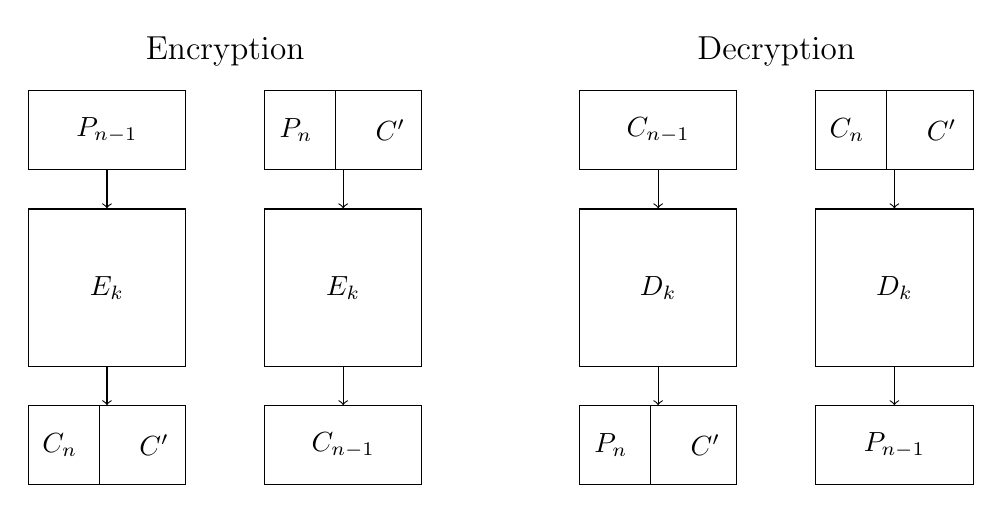
\begin{tikzpicture}[node distance=1cm and 1.5cm, every node/.style={align=center}]
      % Encryption Title
      \node (title1) [font=\large] at (-5,5) {Encryption};

      % Encryption - Left side
      \node (pn1) [draw, minimum width=2cm, minimum height=1cm] at (-6.5,4) {$P_{n-1}$};
      \node (ek1) [draw, minimum width=2cm, minimum height=2cm] at (-6.5, 2) {$E_k$};
      \node (cdash1) at (-5.9, 0) {$C'$};
      \node (cn1) at (-7.1, 0) {$C_n$};
      \node (auxc1) [draw, minimum width=2cm, minimum height=1cm] at (-6.5, 0) {};
      \draw (-6.6, 0.5) -- (-6.6, -0.5);
      \draw[->] (pn1) -- (ek1);
      \draw[->] (ek1) -- (auxc1);

      % Encryption - Right side
      \node (auxp1) [draw, minimum width=2cm, minimum height=1cm] at (-3.5, 4) {};
      \node (pn2) at (-4.1, 4) {$P_n$};
      \node (cdash2) at (-2.9, 4) {$C'$};
      \node (ek2) [draw, minimum width=2cm, minimum height=2cm] at (-3.5, 2) {$E_k$};
      \node (cn2) [draw, minimum width=2cm, minimum height=1cm] at (-3.5,0) {$C_{n-1}$};
      \draw (-3.6, 3.5) -- (-3.6, 4.5);
      \draw[->] (auxp1) -- (ek2);
      \draw[->] (ek2) -- (cn2);

      % Decryption Title
      \node (title2) [font=\large] at (2,5) {Decryption};

      % Decryption - Left side
      \node (cpn1) [draw, minimum width=2cm, minimum height=1cm] at (0.5,4) {$C_{n-1}$};
      \node (dek1) [draw, minimum width=2cm, minimum height=2cm] at (0.5, 2) {$D_k$};
      \node (dcdash1) at (1.1, 0) {$C'$};
      \node (dpn1) at (-0.1, 0) {$P_n$};
      \node (dauxc1) [draw, minimum width=2cm, minimum height=1cm] at (0.5, 0) {};
      \draw (0.4, 0.5) -- (0.4, -0.5);
      \draw[->] (cpn1) -- (dek1);
      \draw[->] (dek1) -- (dauxc1);

      % Decryption - Right side
      \node (dauxp1) [draw, minimum width=2cm, minimum height=1cm] at (3.5, 4) {};
      \node (dcn2) at (2.9, 4) {$C_n$};
      \node (dcdash2) at (4.1, 4) {$C'$};
      \node (dek2) [draw, minimum width=2cm, minimum height=2cm] at (3.5, 2) {$D_k$};
      \node (dpn2) [draw, minimum width=2cm, minimum height=1cm] at (3.5,0) {$P_{n-1}$};
      \draw (3.4, 3.5) -- (3.4, 4.5);
      \draw[->] (dauxp1) -- (dek2);
      \draw[->] (dek2) -- (dpn2);

    \end{tikzpicture}
\end{center}

Bei Ciphertext Stealing wird der vorletzte komplette Block $P_{n-1}$ verschlüsselt und in Teile $C_n$ und $C'$ aufgeteilt. 
Dann wird der letzte Block $P_n$ mit $C'$ gepadded und verschlüsselt. Dieser komplette Block $C_{n-1}$ kommt an die vorletzte Stelle des Ciphertexts und der noch nicht 
verwendete Teil $C_n$ wird angehängt. So kann die Nachricht mit Block Ciphern verschlüsselt werden, ohne sie zu verlängern.

\section{Hash Funktionen}
\section{Byteweise}
\section{RSA}
\section{OAEP}


% \begin{itemize}
% \end{itemize}

% \begin{enumerate}
% \end{enumerate}

% \begin{align*}
% \end{align*}

\chapter{Asymmetrische Kryptographie}

(todo)
% Angewandte_Kryptographie_SoSe2025_part1_v01.pdf, Seite 6ff

\section{Sicherheitsbetrachtungen von RSA}

\section{RSA in der Praxis}

\section{Mathematische Konzepte}

\subsection{Quadratischer Rest}

\subsection{Euler Kriterium und Legendre Symbol}

\subsection{Quadratwurzeln modulo $p$}

\subsection{Quadratwurzeln modulo $n = p \cdot q$}

\section{Rabin public-key encryption}

\chapter{Erzeugung von Primzahlen}

Für public-key-Kryptosysteme benötigt man häufig zufällige große Primzahlen. In der Regel erzeugt man dazu eine natürliche Zahl in der gewünschten Größe und
prüft, ob diese eine Primzahl ist, beispielsweise versucht man diese Zahl $n$ durch alle Primzahlen $\leq \sqrt{n}$ zu teilen, dieses Vorgehensweise ist jedoch sehr 
ineffizient und heißt Probedivision\index{Probedivision}. Sie wird auch in Faktorisierungsalgorithmen mit Primzahlen bis $10^6$ verwendet.

\paragraph{Verteilung der Primzahlen}

Bezeichne $\pi(n)$ die Anzahl der Primzahlen im Intervall $[2, n]$. Es gilt 

$$\pi(n) \sim \frac{n}{\ln(n)} $$


\begin{center}
    \begin{tabular}{ ll } 
        \hline
        $n$ & $\pi(n)$  \\ 
        \hline
                 10 &         4 \\
                100 &        25 \\
               1000 &       168 \\
              10000 &      1229 \\
             100000 &      9592 \\
            1000000 &     78498 \\
           10000000 &    664579 \\
          100000000 &   5761455 \\
         1000000000 &  50847534 \\
        10000000000 & 455052512 \\
        \hline
    \end{tabular}
\end{center}

\paragraph{Abschätzung des Aufwands}

Aus $\pi(n) \sim n / \ln(n)$ folgt: man benötigt wenigstens $\sqrt{n} / \ln(\sqrt{n})$ Probedivisionen, um zu
beweisen, daß eine natürliche Zahl $n$ eine Primzahl ist.
Beispielsweise werden bei RSA Primzahlen verwendet, die aktuell in der Regel größer als
$10^{150}$ sind.\\

Um nun die Primalität für diese Zahl zu beweisen, müßte man insgesamt mehr als
$10^{150/2} / \ln(10^{150/2}) > 5.7 \cdot 10^{72}$ Probedivisionen durchführen -- das ist nicht durchführbar!
Somit sucht man nach effizienteren Verfahren: Primzahltests\index{Primzahltest} stellen mit einer
hohen Wahrscheinlichkeit fest, ob eine Zahl auch eine Primzahl ist (probabilistic primality
tests).
% Angewandte_Kryptographie_SoSe2025_part1_v01.pdf, Seite 34ff

\section{Der Fermat Test}
Der Fermat-Test
- der Test beruht auf dem kleinen Satz von Fermat: Ist n eine Primzahl, so gilt 

$$a^{n-1} \equiv 1  \mod n$$ 

für alle $a \in \mathbb{Z}$ mit gcd($a,n$) = 1.

Somit kann man mit diesem Satz überprüfen, ob eine Zahl zusammengesetzt ist:

\begin{enumerate}
    \item man wählt dazu eine natürliche Zahl $a \in \{1,2, \ldots, n-1\}$
    \item als nächste berechnet man $r = a^{n-1} \mod n$
    \item ist nun $r \neq 1$, so ist $n$ keine Primzahl und zusammengesetzt. Ergibt sich $r = 1$, so kann $n$ eine Primzahl oder zusammengesetzt sein
    \item die Schritte 1 bis 3 müssen für alle Werte von $a$ nun durchlaufen werden, wenn $r = 1$
\end{enumerate}

Es braucht die Festlegung einer ``Sicherheits-Grenze'': Wie oft muss der Algorithmus bei $r = 1$ durchlaufen werden, damit man sicher sein kann, eine Primzahl gefunden 
zu haben?\\
    
\noindent Der Fermat-Test kann zeigen, dass $n$ zusammengesetzt ist, er kann aber nicht beweisen, dass $n$ eine Primzahl ist. \\

\noindent Das Verfahren ist zur Faktorisierung ungeeignet.

\paragraph{Beispiel}
Gegeben: $n = 341 = 11 \cdot 31$,  d.h. $n$ ist keine Primzahl. Wir berechnen für $a = 2$

$$2^{340} \equiv 1 \mod 341,$$

obwohl $n$ zusammengesetzt ist. Für ein anderen $a$, z.B. $a = 3$ haben wir 

$$3^{340} \equiv 56 \mod 341.$$

Im Ergebnis bedeutet das, dass 341 also eine zusammengesetzte Zahl ist und somit nicht prim sein kann.

\section{Carmichael-Zahlen}

Wenn der Fermat-Test für viele Basen $a$ keine Bestätigung für ein zusammengesetztes $n$
gefunden hat, ist es wahrscheinlich, dass $n$ eine Primzahl ist.
Es existieren aber natürliche Zahlen, deren Eigenschaft ist, dass sie zusammengesetzt sind,
das jedoch nicht mit dem Fermat-Test gezeigt werden kann. \\

Sei $n$ eine ungerade zusammengesetzte Zahl und es gilt für eine ganze Zahl $a$ folgende
Kongruenz

$$a^{n-1} \equiv 1 \mod n,$$

so nennt man $n$ eine Pseudoprimzahl zur Basis $a$. Sei $n$ nun eine Pseudoprimzahl zur Basis $a$ für alle ganzen Zahlen $a$ mit gcd($a,n$) = 1. Dann
heißt $n$ Carmichael-Zahl\index{Carmichael-Zahl}. 

\paragraph{Beispiel} für eine Carmichael-Zahl: $561 = 3 \cdot 11 \cdot 17$.

\paragraph{Eigenschaften} Eine ungerade zusammengesetzte Zahl $n \geq 3$ ist eine Carmichael-Zahl, wenn genau
diese zwei Bedingungen gelten:
\begin{enumerate}
    \item $n$ ist quadratfrei, d.h. $n$ hat keinen mehrfachen Primteiler
    \item $p - 1$ teilt $n - 1$ für alle Primteiler $p$ von $n$
\end{enumerate}

Somit folgt, dass jede Carmichael-Zahl ein Produkt von mindestens drei unterschiedlichen
Primzahlen ist. Daher wissen wir auch, dass unendlich viele Carmichael-Zahlen existieren.

\section{Der Miller-Rabin Test}

Im Gegensatz zum Fermat-Test findet der Miller-Rabin-Test nach ``ausreichend'' vielen
Durchläufen für jede natürliche Zahl heraus, ob diese zusammengesetzt ist. \\


\noindent Sei $n$ eine natürliche ungerade Zahl mit $s = \max\{r \in \mathbb{N} | 2^r \text{ teilt } n-1\}$.
Damit ist $2^s$ die größte Potenz, die $n-1$ teilt oder anders ausgedrückt: es gibt ein ungerades $d \in \mathbb{Z}$, sodass $n - 1 = 2^s \cdot d$.

\begin{theorem}
    Ist $n$ eine Primzahl und $a$ eine zu $n$ teilerfremde ganze Zahl, so gilt mit den
obigen Bezeichnungen entweder
    \begin{enumerate}
        \item $a^d \equiv 1 \mod n$
        \item$a^{2^r \cdot d} \equiv -1 \mod n$
    \end{enumerate}
\end{theorem}

Mindestens eine der Bedingungen muss erfüllt sein, dass $n$ eine Primzahl ist. Weiters gilt, $n$ ist keine Primzahl (also zusammengesetzt) g.d.w. man eine ganze zu $n$ 
teilerfremde Zahl $a$ findet, für die weder die Bedingung (1) noch (2) für ein $r \in \{0, 1, \ldots, s-1\}$ gilt.
Dann wird $a$ Zeuge gegen die Primalität von $n$ genannt.

\paragraph{Beispiel}
Sei $n = 561$ und $a = 2$. Wir behaupten $a$ ist eine Zeuge gegen die Primalität von $n$:

Wir berechnen $s = 4$ und wählen $d = 35$, dann gilt

\begin{align*}
    2^{35} &\equiv 263 \mod 561 \\
    2^{2\cdot 35} &\equiv 166 \mod 561 \\ 
    2^{4\cdot 35} &\equiv 67 \mod 561 \\
    2^{8\cdot 35} &\equiv 1 \mod 561
\end{align*}

Also ist 561 keine Primzahl nach vorhergehenden Theorem.

\paragraph{Abschätzung der Anzahl der Zeugen gegen eine Primalität einer Zahl $n$}

\begin{theorem}
Sei $n \geq 3$ eine ungerade zusammengesetzte Zahl, so gibt es in der Menge
$\{1,2, \ldots, n-1\}$ höchstens $(n-1)/4$ Zahlen, die zu $n$ teilerfremd sind und keine Zeugen gegen die
Primalität von $n$ sind.
\end{theorem}

Für einen Beweis: vgl. Buchmann J., Einführung in die Kryptographie, 3. Auflage, S. 127 ff.

\paragraph{Beispiel}: Bestimmung aller Zeugen gegen eine Primalität der Zahl $n$.
Sei $n = 15$, es ist $n-1 = 14 = 2 \cdot 7$, daraus folgt: $s = 1$ und $d = 7$. Eine zu 15 teilerfremde Zahl $a$ ist genau dann Zeuge gegen die Primzahleigenschaft
von $n$ wenn $a^7 \mod 15 \neq \pm 1$ gilt.

In einer tabellarischen Übersicht:


\begin{center}
    \begin{tabular}{ ccc ccc ccc } 
        \hline
        $a$ & 1 & 2 & 4 & 7 & 8 & 11 & 13 & 14 \\ 
        \hline
        $a^{14} \mod 15$ &  1 &  4 &  1 &  4 &  4 &  1 &  4 &  1 \\
        $a^{ 7} \mod 15$ &  1 &  8 &  4 & 13 &  2 & 11 &  7 & 14 \\ 
        \hline
    \end{tabular}
\end{center}

Die Anzahl der zu 15 teilerfremden Zahlen in $\{1, 2,\dots,14\}$, die keine Zeugen gegen die
Primalität von $n = 15$ sind, beläuft sich auf $2 \leq (15 - 1)/4 = 3.5$.

\paragraph{Anwendung} des Miller-Rabin-Tests auf eine ungerade Zahl $n$

\begin{itemize}
    \item man wählt zufällig und gleichverteilt eine Zahl aus der Menge $\{2,3,\dots, n-1\}$
    \item ist der gcd($a,n$) > 1, so ist $n$ zusammengesetzt
    \item ist der gcd($a,n$) = 1, so testet man $a^d, a^{2d}, a^{2^2d}, \ldots, a^{2^{s-1}d}$
    \item findet man nun einen Zeugen gegen die Primalität von $n$, dann wurde gezeigt, dass $n$ zusammengesetzt ist
    \item die Wahrscheinlichkeit dafür, dass $n$ zusammengesetzt ist und man keinen Zeugen findet, beläuft sich nach obigen Theorem auf höchstens $0.25$.
\end{itemize}

Ist $n$ zusammengesetzt, so findet man bei der Iteration des Miller-Rabin-Tests mit $t$ Durchläufen mit einer Wahrscheinlichkeit von höchstens $frac14t$ keinen Zeugen 
gegen die Primalität von $n$.

\paragraph{Beispiel} nach 10 Durchläufen ergibt sich eine Wahrscheinlichkeit von $frac14 10$, das entspricht ungefähr einer $0.0001$-prozentigen Wahrscheinlichkeit, 
dass man keinen Zeugen gegen die Primzahleigenschaft von $n$ findet.

\section{Verfahren zur zufälligen Wahl von Primzahlen}

Beim Verfahren für die Erzeugung einer zufälligen $k$-Bit-Primzahl: dabei wird zuerst eine zufällige und ungerade $k$-Bit-Zahl $n$ generiert.
Davon wird das erste und letzte Bit wird auf 1 gesetzt, die restlichen $k-2$ Bits werden zufällig und gleichverteilt gesetzt. 
Jetzt wird überprüft, ob $n$ eine Primzahl ist:
\begin{itemize}
    \item ist $n$ durch eine Primzahl unter einer gewissen Schranke $B$ (in der Regel wird $B = 10^6$ gesetzt) teilbar? Die Primzahlen werden in einer Tabelle vorgehalten.
    \item wird dabei kein Teiler von $n$ gefunden, so wird der Miller-Rabin-Test mit $t$ Wiederholungen ( mit $t \geq 1$ als entsprechender Sicherheitsparameter) auf $n$ 
    angewendet
    \item wird dabei kein Zeuge gegen die Primzahleigenschaft von $n$ gefunden, so gilt $n$ nun als Primzahl (mit der Sicherheit $\frac{t}{4}$).
    \item ansonsten muß der gesamte Test mit einer anderen Zahl $n'$ wiederholt werden
\end{itemize}

Die Auswahl der Schranke $B$ hängt von dem Verhältnis der Ausführungszeiten einer
Probedivision und eines Miller-Rabin-Tests auf der verwendeten Hard- bzw. Software-Plattform ab.
\chapter{Hash-Funktionen}

Die Anforderungen an eine kryptographische Hashfunktion sind:
\begin{itemize}
    \item Kompression, d.h. ein beliebig langer Input wird auf einen Output fixer Länge gemappt
    \item Einwegfunktion (preimage resistance), d.h. gegeben $y = h(x)$ ist es schwierig, das verwendete $x$ zu bestimmen
    \item Schwache Kollisionsresistenz (2nd preimage resistance), d.h. gegeben $x$ mit $y = h(x)$ ist es schwierig, ein $x' \neq x$ zu finden, so dass $h(x) = h(x')$
    \item Starke Kollisionsresistenz (collision resistance), d.h. es ist schwierig, zwei $x$ und $x'$ zu finden, mit $x \neq x'$, so dass $h(x) = h(x')$
\end{itemize}

\section{Konstruktion}

Grundsätzlich sind für eine Hashfunktion zwei Komponenten nötig, eine Kompressionsfunktion, die längere Inputs auf die gewünschte Länge komprimieren, und ein Domain 
Extender, der aus Funktionen mit Eingaben fester Länge Funktionen mit Eingabe beliebiger Länge macht.

\paragraph{Kompressionsfunktionen} haben für einen fixen Input $m$ einen fixen Output $n$ mit $|m| > |n|$.

Es wird entweder eine eigens für den Hash geschriebene Funktion verwendet, z.B. bei MD5 und SHA-1, SHA-2, SHA-3, oder es wird ein Blockcipher eingesetzt. Bei einem 
Blockcipher wird ein Input der Länge $k+l$ (Länge des Schlüssels und Länge des Klartexts) auf einen Input der Länge $l$ gemappt. \\

Die zwei häufigsten Konstruktionen sind
\begin{itemize}
    \item Davis-Meyer: $h(x, y) = E_y(x) \oplus y$
    \item Miyaguchi-Preneel: $h(x, y) = E_x(y) \oplus x \oplus y$
\end{itemize}



\paragraph{Domain Extender} machen aus einer Funktion, die nur Inputs mit einer fixen Länge $n$ nimmt, eine Funktion die Inputs mit beliebiger Länge nimmt. 

Mehr oder weniger alle modernen Hashfunktionen folgen diesem Prinzip:

\begin{enumerate}
    \item Input wird in Blöcke $x_1, \ldots, x_n$ gleicher Länge aufgespalten
    \item Jeder Block dient als Input einer Einweg-Kompressionsfunktion $f$
    \item Input des $i$-ten Funktionsaufrufs sind das vorherige Ergebnis $h_{i-1}$ und der $i$-te Nachrichtenblock $x_i$
    \begin{itemize}
        \item $h_i = f(h_{i-1}, x_i)$
        \item $h(x) = h_{n+1}$ für eine Nachricht mit {n} Blöcken
        \item $h_i$ ist der interne Zustand der Hashfunktion
    \end{itemize}
    \item Ist die verwendete Funktion $f$ kollisionsresistent, so gilt das auch für $h$
    \item Im letzten Block der zu hashenden Nachricht wird die Länge der Originalnachricht angehängt, damit gleich endende aber unterschiedlich lange Nachrichten 
    unterschiedliche Hashwerte ergeben, z.B. \verb|Foo0| vs. \verb|Foo00|
    \item Grundproblem der Konstruktion: Length Extension Attack
    \begin{itemize}
        \item Kompletter interner State ist in Hashwert enthalten
        \item Falls MAC Konstruktion der Form H(key||Nachricht) ist, kann leicht Hashwert für verlängerte Nachricht konstruiert werden
    \end{itemize}
\end{enumerate}

\section{Algebraische Hashfunktionen}

In der Praxis werden aus Geschwindigkeitsgründen hauptsächlich Hashfunktionen
basierend auf logischen Funktionen verwendet. Algebraische Funktionen sind kaum verbreitet, sie basieren auf ähnlichen Argumentationen wie
Public-Key Kryptographie (vgl. AES vs. RSA), also z.B. dem DLP (Discrete Logarithm Problem). Für die Hashfunktion gilt 

$$h(x) = g^x \mod p,$$

wobei das Umkehren der Funktion äquivalent zum Lösen des diskreten Logarithmusproblems ist.
Es gibt auch Hashfunktionen basierend auf RSA

$$H(x) = g^x \mod n (\text{mit } n = p\cdot q),$$

wo das Umkehren der Funktion äquivalent zum Lösen des RSA Problems ist.

\section{MD5} wurde 1991 von Ron Rivest als verbesserter Nachfolger zu MD4 erfunden.

\begin{itemize}
    \item 1996 erste Fehler entdeckt, 2004 weitere Schwachstellen gefunden
    \item 2007 Methoden vorgestellt, um 2 Dateien mit selber MD5 Checksumme zu erzeugen
    \item 2008 gefälschte SSL Zertifikate mit dieser Methode erzeugt
    \item 2008: ``Software developers, Certification Authorities, website owners, and users should avoid using the MD5 algorithm in any capacity. As previous research 
    has demonstrated, it should be considered cryptographically broken and unsuitable for further use.'' -- US-CERT, \url{http://www.kb.cert.org/vuls/id/836068}
\end{itemize}

Die Funktion erzeut in 64 Operationen (in 4 Runden zu je 16 Operationen) einen Output der Länge 128.

\begin{enumerate}
    \item Nachricht wird in 512 Bit große Blöcke aufgespalten und gepadded (siehe Kapitel ``Padding'')
    \item der interne State hat 128 Bit, wird in 4 32-Bit Wörtern gehalten. Er wird mit \verb|01 23 45 67|, \verb|89 ab cd ef|, \verb|fe dc ba 98|, \verb|76 54 32 10|, 
    sogenannte ``nothing up my sleeve'' numbers
    \item es gibt eine additive Rundenkonstante: in Runde $i$ wird $K_i = 2^{32}\cdot|\sin(i)|$ addiert 
    \item Alle 16 Operationen wechselt die Rundenfunktion ($F$, $G$, $H$, $I$)
    \begin{itemize}
        \item F(X,Y,Z) = (X and Y) or (not X and Z)
        \item G(X,Y,Z) = (X and Z) or (Y and not Z)
        \item H(X,Y,Z) = X $\oplus$ Y $\oplus$ Z
        \item I(X,Y,Z) = Y $\oplus$ (X or not Z)
    \end{itemize}
    \item Jede Runde um anderen Offset zirkulär geshiftet
\end{enumerate}

\begin{figure}[h]
    \includegraphics[width=0.4\textwidth]{figures/fig09-md5}
    \centering
    \caption{MD5 Operation, die 64 Mal wiederholt wird}
\end{figure}


\section{SHA (Secure Hash Algorithm)}

1993 wurde SHA-0 veröffentlicht, 1995 dann der verbesserte SHA-1 und 2001 SHA-2. Das NIST hat SHA-3 ausgeschrieben, das Ende des Auswahlprozesses war 2012 (vgl. AES).
Dann wurde Keccak als SHA-3 2015 standardisiert. \\

\paragraph{SHA-1}
Der SHA-1 mit voller Rundenzahl gilt seit 2005 als unsicher. Kollisionen können mit $2^{63}$ Operationen erzeugt werden, 2008 wurde die Zahl auf $2^{51}$ verringert.
Seit 2017 sind Kollisionen in 2 validen PDF Dokumenten konstruierbar. \\

Er erzeugt einen 160 Bit Output und basiert auf denselben Grundideen wie MD4 und MD5:

\begin{itemize}
    \item Nachricht ebenfalls in 512-Bit Blöcke gespalten
    \item es gibt 80 Runden, alle 20 Runden wechselt die Rundenfunktion
    \begin{enumerate}
        \item F(X,Y,Z) = (X and Y) or (not X and Z) (ident zu MD5)
        \item G(X,Y,Z) = X $\oplus$ Y $\oplus$ Z (ident zu H aus MD5)
        \item H(X,Y,Z) = (X and Y) or (X and Z) or (Y and Z)
        \item I(X,Y,Z) = G (sic)
    \end{enumerate}
    \item es gibt 4 Rundenkonstanten
    \begin{enumerate}
        \item $K_1 = 230 \cdot \sqrt(2)$ 
        \item $K_2 = 230 \cdot \sqrt(3)$
        \item $K_3 = 230 \cdot \sqrt(5)$
        \item $K_4 = 230 \cdot \sqrt(10)$
    \end{enumerate}
    \item In jeder Runde um 30 zirkulär geshiftet
\end{itemize}

\paragraph{SHA-2} beschreibt eine Familie an Hashfunktionen, die die Algorithmen SHA-224, SHA-256, SHA-384, SHA-512, SHA-512/224 und SHA-512/256. Sie sind im FIPS 
(Federal Information Processing Standards) PUB-180-4 beschrieben.


\begin{center}
    \begin{tabular}{ llll } 
        \hline
        Algorithmus & Ausgabegröße (Bit) & Interne Blockgröße (Bit) & basiert auf \\ 
        \hline
        SHA-224     & 224 &  512 & SHA-256\\
        SHA-256     & 256 &  512 & SHA-256\\
        SHA-384     & 384 & 1024 & SHA-512\\
        SHA-512     & 512 & 1024 & SHA-512\\
        SHA-512/224 & 224 & 1024 & SHA-512\\
        SHA-512/256 & 256 & 1024 & SHA-512\\
        \hline
    \end{tabular}
\end{center}

\subparagraph{SHA-224}: Kürzere Version von SHA-256 mit 224 Bit Ausgabelänge. Geeignet, wenn Speicher knapp ist, z.B. constraint devices (Memory).
\subparagraph{SHA-256}: Der meistverwendete SHA-2-Algorithmus. Standard für viele Anwendungen (z. B. TLS, digitale Signaturen)
\subparagraph{SHA-384}: Abgespeckte Version von SHA-512 mit anderer Initialisierung und kürzerer Ausgabe.
\subparagraph{SHA-512}: Sicherste (längste) Standardvariante mit 512 Bit Ausgabelänge.
\subparagraph{SHA-512/224} (constraint devices (Memory)), siehe SHA-512/256.  
\subparagraph{SHA-512/256} (allg. Sicherheit): Truncate-Versionen von SHA-512 mit kürzerer Ausgabelänge. Bietet eine Kombination aus höherer
Sicherheit (wegen 1024-Bit Blockgröße) und kürzeren Hashes.


\subparagraph{Merkle-Damgard}

Die Merkle-Damg\r{a}rd-Konstruktion (auch Merkles Meta-Verfahren) ist eine Methode zur Konstruktion von kryptographischen Hash-Funktionen, die auf Arbeiten von 
Ralph Merkle und Ivan Damg\r{a}rd zurückgeht.
Gegeben ist eine kollisionsresistente Kompressionsfunktion $f: \{0, 1\}^{a+b} \to \{0, 1\}^b$. Durch die Anwendung der Merkle-Damg\r{a}rd-Konstruktion ergibt sich daraus 
eine kollisionssichere Hash-Funktion $h: \{0, 1\}^* \to \{0, 1\}^b$, die beliebig lange Nachrichten auf einen Hashwert abbilden.

\begin{figure}[h]
    \includegraphics[width=0.9\textwidth]{figures/fig10-merkle-damgard}
    \centering
    \caption{Merkle-Damgard Hash}
\end{figure}

\begin{enumerate}
    \item Padding (Auffüllen): Die Eingabenachricht wird so erweitert, dass ihre Länge ein Vielfaches der Blockgröße ist. Dabei wird meist die ursprüngliche 
    Nachrichtenlänge am Ende angehängt.
    \item Aufteilung in Blöcke: Die aufgefüllte Nachricht wird in gleichgroße Blöcke unterteilt.
    \item Initialisierung: Ein fester Startwert (IV = Initialization Vector) wird gesetzt.
    \item Iterative Verarbeitung: Für jeden Block wird die Kompressionsfunktion angewendet:
    \begin{itemize}
        \item Eingabe: der aktuelle Block + der Ausgabewert des vorherigen Schritts
        \item Ausgabe: ein neuer Zwischenwert
    \end{itemize}
    \item Finales Ergebnis: Der Ausgabewert nach dem letzten Block ist der Hash-Wert.
\end{enumerate}

\subsection{SHA-3}


2007 begann das NIST mit der Ausschreibung für einen Nachfolger von SHA-2. Am 2.10.2012 wurde Keccak (von Guido
Bertoni, Joan Daemen, Gilles Van Assche und Michaël Peeters) als Sieger verkündet und stellt die Basis für SHA-3 dar.

\begin{itemize}
    \item Verwendet im Unterschied zur bisherigen SHA Familie eine sog. ``Sponge'' Konstruktion: ein 3-dimensionaler innerer Zustand ($5\times 5\times w$ -Bit Wörter; 
    bei $w =64$ sind das 1.600 Bits)
    \item Permutation: 24 Runden, 5 Schritte ($\theta, \rho, \pi, \chi, \iota$)
    \item Zuerst wird der zu hashende Text zur Gänze ``aufgesogen'' (absorbing phase)
    \item Danach der Hash gewünschter Länge ``ausgepresst'' (squeezing phase)
    \item Das ergibt Hashlängen von 224 bis 512 Bit (theoretisch aber beliebig lange, bis maximal 1.600); wird auch als Capacity Wert bezeichnet
\end{itemize}

\paragraph{Phasen}

\begin{figure}[h]
    \includegraphics[width=0.75\textwidth]{figures/fig11-sponge}
    \centering
    \caption{SHA-3, Absorbing- und Squeezing Phase}
\end{figure}

\subparagraph{Absorbieren} Eingabedaten werden in Blöcke unterteilt.
Jeder Block wird mit dem internen Zustand (einer Art Speicher) verXORt.
Danach wird eine Permutation ($f$) auf den Zustand angewendet.

\subparagraph{Auspressen} Nachdem alle Eingabeblöcke
absorbiert wurden, wird ein Teil des internen Zustands als Ausgabe extrahiert.
Bei langen Ausgaben (z.B. SHAKE-Funktionen) wird $f$ mehrfach ausgeführt, um mehr Output zu generieren.

\paragraph{State} Der interne Zustand in KECCAK hat die Breite $b=1600$ Bits (für SHA-3). Dieser Zustand ist aufgeteilt in ein 3D-Array mit
Dimensionen $5 \times 5 \times w$, wobei $w = 64$ bits. Jede Zelle $A[x][y]$ ist ein sogenanntes ``lane'' mit 64 Bits. 

\paragraph{Parameter}

Neben der Größe des States $b$, gibt es noch die Parameter

\begin{itemize}
    \item Rate $r$, wie viele Bits pro Sekunde verarbeitet werden können 
    \item Capacity $c$, wie groß die Sicherheitsreserve ist, sie berechnet sich als $c = b - r$. Bei Kapazität $c$  bietet der Algorithmus $c/2$ Bit Widerstand gegen 
    Kollisions- und Preimage-Attacken. 
\end{itemize}

Für den SHA-256 haben die Parameter $(b, r, c)$ dem Wert $(1600, 1088, 512)$.

\paragraph{Permutationsfunktion} KECCAK-f hat 24 Runden mit je 5 Steps:
\begin{enumerate}
    \item $\theta$ (theta) mischt jede Lane mit einer XOR-Mischung ihrer Spaltennachbarn.
    \item $\rho$ (rho) rotiert die Bits jeder Lane um einen bestimmten Wert.
    \item $\pi$ (pi) permutiert die Positionen der Lanes im $5\times 5$-Gitter.
    \item $\chi$ (chi) führt eine nichtlineare XOR-Maske aus, basierend auf anderen Werten in der Zeile.
    \item $\iota$ (iota) fügt einen Rundenkonstanten hinzu (zum Schutz vor symmetrischen Mustern).
\end{enumerate}

\noindent Diese Schritte garantieren Diffusion, Konfusion und Nichtlinearität, wie bei modernen
Blockchiffren.

\paragraph{Padding} Um sicherzustellen, dass die Nachricht gleichmäßig in $r$-Bit-Blöcke aufgeteilt werden
kann, ist ein Padding erforderlich. SHA-3 verwendet das Muster 100...001 (01 Padding), ein Bit mit Wert 1 wird gefolgt von null oder mehr 0-Bits (maximal $r-1$) und 
einem letzten 1-Bit.

\paragraph{XOFs} (Extendable Output Functions) basieren auf KECCAK und geben beliebig viele Ausgabebits zurück (nicht nur 256 oder 512).
Sie sind sehr flexibel für Anwendungen wie:
\begin{itemize}
    \item Key Derivation Function (KDF)
    \item Authentifizierung
    \item PQC Signaturen (z. B. SPHINCS+, Dilithium)
\end{itemize}

SHAKE bezeichnet den KECCAK Algorithmus, der er ein anderes Padding (1111 statt 01) und eine variable Ausgabelänge hat.


\section{Angriffe}

Sei $n$ die Länge des Outputs. Die Angriffe auf Hashfunktionen können wie folgt kategorisiert werden:

\begin{itemize}
    \item Angriff auf die Eigenschaft als Einwegfunktion: Idealerweise Komplexität von $O(2^n)$
    \item Angriff auf die schwache Kollisionsresistenz: Idealerweise Komplexität von $O(2^n)$ 
    \item Angriff auf die starke Kollisionsresistenz: Idealerweise Komplexität von $1.2\cdot 2^{n/2}$ (Geburtstagsparadoxon)
\end{itemize}

Generell gilt, ein Aufwand von $2^{80}$ ist ``schwierig''.

\paragraph{MD5} ist gebrochen.
\paragraph{SHA-1} ist gebrochen.
\paragraph{SHA-2} 

\begin{itemize}
    \item Output: 224/256/384/512 Bit
    \item Struktur: Merkle-Damgard
    \item Theoretische Angriffe auf rundenreduzierte Versionen bekannt
\end{itemize}

\paragraph{SHA-3}

\begin{itemize}
    \item Output: 224/256/384/512 Bit
    \item Struktur: Sponge
\end{itemize}

\subsection{BEAST Attack}

Steht für \textbf{B}rowser \textbf{E}xploit \textbf{A}gainst \textbf{S}SL/\textbf{T}LS.
\begin{itemize}
    \item MitM Angriff und Chosen Plaintext Attack
    \item Record Splitting
    \item CBC Mode mit unsicherer IV-Generierung
    \item Beschrieben in CVE-2011-3389
    \item TLS1.0
\end{itemize}

Der BEAST-Angriff nutzt die Tatsache aus, dass bei TLS 1.0 der
Initialisierungsvektor (IV) für die nächste Nachricht vorhersehbar ist:
Er ist nämlich der letzte verschlüsselte Block der vorherigen Nachricht.

Dadurch kann ein Angreifer über sogenannte Chosen-Plaintext-Angriffe (d. h. gezielt eingefügte Daten) Rückschlüsse auf vertrauliche
Inhalte wie Cookies ziehen. \\

\noindent Damalige temporäre Workarounds
\begin{itemize}
    \item RC4
    \item 0-length Packets
    \item 1/n-1 Packet-Splitting: 
    \begin{itemize}
        \item Erster Record (1 Byte): Enthält nur ein harmloses Byte (z. B. ein Leerzeichen oder ein kontrolliertes Zeichen).
        \item Zweiter Record (n-1 Bytes): Enthält den Rest der eigentlichen Nachricht (z.B. HTTP-Headers, Cookies usw.).
    \end{itemize}
\end{itemize}
 

\begin{figure}[h]
    \includegraphics[width=0.9\textwidth]{figures/fig12-beast-attack-1}
    \centering
    \caption{How it should work: Proper encryption using a block cipher in CBC mode}
\end{figure}
\begin{figure}[h]
    \includegraphics[width=0.9\textwidth]{figures/fig13-beast-attack-2}
    \centering
    \caption{The underlying vulnerability: A record splitting attack against TLS 1.0}
\end{figure}
\begin{figure}[h]
    \includegraphics[width=0.9\textwidth]{figures/fig14-beast-attack-3}
    \centering
    \caption{The BEAST exploit: A chosen boundary attack combined with record splitting}
\end{figure}
\input{chapters/7-integer-factorisation}
\input{chapters/8-signatures}

%%% backmatter %%%
\backmatter

% \bibliographystyle{plain}
% \bibliography{bibliography}
\printindex

\end{document}

